% !TeX spellcheck = pl_PL
%%%%%%%%%%%%%%%%%%%%%%%%%%%%%%%%%%%%%%%%%%%
%                                        %
% Szablon pracy dyplomowej inzynierskiej %
% zgodny  z aktualnymi  przepisami  SZJK %
%                                        %
%%%%%%%%%%%%%%%%%%%%%%%%%%%%%%%%%%%%%%%%%%
%                                        %
%  (c) Krzysztof Simiński, 2018-2023     %
%                                        %
%%%%%%%%%%%%%%%%%%%%%%%%%%%%%%%%%%%%%%%%%%
%                                        %
% Najnowsza wersja szablonów jest        %
% podstępna pod adresem                  %
% github.com/ksiminski/polsl-aei-theses  %
%                                        %
%%%%%%%%%%%%%%%%%%%%%%%%%%%%%%%%%%%%%%%%%%
%
%
% Projekt LaTeXowy zapewnia odpowiednie formatowanie pracy,
% zgodnie z wymaganiami Systemu zapewniania jakości kształcenia.
% Proszę nie zmieniać ustawień formatowania (np. fontu,
% marginesów, wytłuszczeń, kursywy itd. ).
%
% Projekt można kompilować na kilka sposobów.
%
% 1. kompilacja pdfLaTeX
%
% pdflatex main
% bibtex   main
% pdflatex main
% pdflatex main
%
%
% 2. kompilacja XeLaTeX
%
% Kompilatacja przy użyciu XeLaTeXa różni się tym, że na stronie
% tytułowej używany jest font Calibri. Wymaga to jego uprzedniego
% zainstalowania.
%
% xelatex main
% bibtex  main
% xelatex main
% xelatex main
%
%
%%%%%%%%%%%%%%%%%%%%%%%%%%%%%%%%%%%%%%%%%%%%%%%%%%%%%
% W przypadku pytań, uwag, proszę pisać na adres:   %
%      krzysztof.siminski(małpa)polsl.pl            %
%%%%%%%%%%%%%%%%%%%%%%%%%%%%%%%%%%%%%%%%%%%%%%%%%%%%%
%
% Chcemy ulepszać szablony LaTeXowe prac dyplomowych.
% Wypełniając ankietę spod poniższego adresu pomogą
% Państwo nam to zrobić. Ankieta jest całkowicie
% anonimowa. Dziękujemy!


% https://docs.google.com/forms/d/e/1FAIpQLScyllVxNKzKFHfILDfdbwC-jvT8YL0RSTFs-s27UGw9CKn-fQ/viewform?usp=sf_link
%
%%%%%%%%%%%%%%%%%%%%%%%%%%%%%%%%%%%%%%%%%%%%%%%%%%%%%%%%%%%%%%%%%%%%%%%%%

%%%%%%%%%%%%%%%%%%%%%%%%%%%%%%%%%%%%%%%%%%%%%%%
%                                             %
% PERSONALIZACJA PRACY – DANE PRACY           %
%                                             %
%%%%%%%%%%%%%%%%%%%%%%%%%%%%%%%%%%%%%%%%%%%%%%%

% Proszę wpisać swoje dane w poniższych definicjach.

% TODO
% dane autora
\newcommand{\FirstNameAuthor}{Krzysztof}
\newcommand{\SurnameAuthor}{Grądek}
\newcommand{\IdAuthor}{300362}   % numer albumu  (bez $\langle$ i $\rangle$)

% drugi autor:
%\newcommand{\FirstNameCoauthor}{Imię}   % Jeżeli jest drugi autor, to tutaj należy podać imię.
%\newcommand{\SurnameCoauthor}{Nazwisko} % Jeżeli jest drugi autor, to tutaj należy podać nazwisko.
%\newcommand{\IdCoauthor}{$\langle$wpisać właściwy$\rangle$}  % numer albumu drugiego autora (bez $\langle$ i $\rangle$)
% Gdy nie ma drugiego autora, należy zostawić poniższe definicje puste, jak poniżej. Gdy jest drugi autor, należy zakomentować te linie.
\newcommand{\FirstNameCoauthor}{} % Jeżeli praca ma tylko jednego autora, to dane drugiego autora zostają puste.
\newcommand{\SurnameCoauthor}{}   % Jeżeli praca ma tylko jednego autora, to dane drugiego autora zostają puste.
\newcommand{\IdCoauthor}{}  % Jeżeli praca ma tylko jednego autora, to dane drugiego autora zostają puste.
%%%%%%%%%%

\newcommand{\Supervisor}{dr inż. Krzysztof Jaskot}     % dane promotora (bez $\langle$ i $\rangle$)
\newcommand{\Title}{Budowa mapy otoczenia z wykorzystaniem robota mobilnego}           % tytuł pracy po polsku
\newcommand{\TitleAlt}{Construction of an Environment Map Using a Mobile Robot}                     % thesis title in English
\newcommand{\Program}{Automatyka i Robotyka}            % kierunek studiów  (bez $\langle$ i $\rangle$)
\newcommand{\Specialisation}{Technologie Informacyjne}     % specjalność  (bez $\langle$ i $\rangle$)
\newcommand{\Departament}{Katedra Automatyki i Robotyki}        % katedra promotora  (bez $\langle$ i $\rangle$)

% Jeżeli został wyznaczony promotor pomocniczy lub opiekun, proszę go/ją wpisać ...
%\newcommand{\Consultant}{$\langle$stopień naukowy imię i nazwisko$\rangle$} % dane promotora pomocniczego, opiekuna (bez $\langle$ i $\rangle$)
% ... w przeciwnym razie proszę zostawić puste miejsce jak poniżej:
\newcommand{\Consultant}{} % brak promotowa pomocniczego / opiekuna

% koniec fragmentu do modyfikacji
%%%%%%%%%%%%%%%%%%%%%%%%%%%%%%%%%%%%%%%%%%


%%%%%%%%%%%%%%%%%%%%%%%%%%%%%%%%%%%%%%%%%%%%%%%
%                                             %
% KONIEC PERSONALIZACJI PRACY                 %
%                                             %
%%%%%%%%%%%%%%%%%%%%%%%%%%%%%%%%%%%%%%%%%%%%%%%

%%%%%%%%%%%%%%%%%%%%%%%%%%%%%%%%%%%%%%%%


%%%%%%%%%%%%%%%%%%%%%%%%%%%%%%%%%%%%%%%%%%%%%%%
%                                             %
% PROSZĘ NIE MODYFIKOWAĆ PONIŻSZYCH USTAWIEŃ! %
%                                             %
%%%%%%%%%%%%%%%%%%%%%%%%%%%%%%%%%%%%%%%%%%%%%%%



\documentclass[a4paper,twoside,12pt]{book}
\usepackage[utf8]{inputenc}                                      
\usepackage[T1]{fontenc}  
\usepackage{amsmath,amsfonts,amssymb,amsthm}
\usepackage[british,polish]{babel} 
\usepackage{indentfirst}
\usepackage{xurl}
\usepackage{xstring}
\usepackage{ifthen}



\usepackage{ifxetex}

\ifxetex
	\usepackage{fontspec}
	\defaultfontfeatures{Mapping=tex—text} % to support TeX conventions like ``——-''
	\usepackage{xunicode} % Unicode support for LaTeX character names (accents, European chars, etc)
	\usepackage{xltxtra} % Extra customizations for XeLaTeX
\else
	\usepackage{lmodern}
\fi



\usepackage[margin=2.5cm]{geometry}
\usepackage{graphicx} 
\usepackage{hyperref}
\usepackage{booktabs}
\usepackage{tikz}
\usepackage{pgfplots}
\usepackage{mathtools}
\DeclareMathOperator*{\argmin}{arg\,min}
\usepackage{geometry}
\usepackage{subcaption}   % subfigures
\usepackage[page]{appendix} % toc,
\renewcommand{\appendixtocname}{Dodatki}
\renewcommand{\appendixpagename}{Dodatki}
\renewcommand{\appendixname}{Dodatek}

\usepackage{csquotes}
\usepackage[natbib=true,backend=bibtex,maxbibnames=99]{biblatex}  % kompilacja bibliografii BibTeXem
%\usepackage[natbib=true,backend=biber,maxbibnames=99]{biblatex}  % kompilacja bibliografii Biberem
\bibliography{biblio}

\usepackage{ifmtarg}   % empty commands  

\usepackage{setspace}
\onehalfspacing


\frenchspacing

%%%%%%%%%%%%%%%%%%%%%%%%%%%%%%%%%%
% środowiska dla definicji, twierdzenia, przykładu
\usepackage{amsthm}

\newtheorem{Definition}{Definicja}
\newtheorem{Example}{Przykład}
\newtheorem{Theorem}{Twierdzenie}
%%%%%%%%%%%%%%%%%%%%%%%%%%%%%%%%%%

%%%% TODO LIST GENERATOR %%%%%%%%%

\usepackage{color}
\definecolor{brickred}      {cmyk}{0   , 0.89, 0.94, 0.28}

\makeatletter \newcommand \kslistofremarks{\section*{Uwagi} \@starttoc{rks}}
  \newcommand\l@uwagas[2]
    {\par\noindent \textbf{#2:} %\parbox{10cm}
{#1}\par} \makeatother


\newcommand{\ksremark}[1]{%
{%\marginpar{\textdbend}
{\color{brickred}{[#1]}}}%
\addcontentsline{rks}{uwagas}{\protect{#1}}%
}

\newcommand{\comma}{\ksremark{przecinek}}
\newcommand{\nocomma}{\ksremark{bez przecinka}}
\newcommand{\styl}{\ksremark{styl}}
\newcommand{\ortografia}{\ksremark{ortografia}}
\newcommand{\fleksja}{\ksremark{fleksja}}
\newcommand{\pauza}{\ksremark{pauza `--', nie dywiz `-'}}
\newcommand{\kolokwializm}{\ksremark{kolokwializm}}
\newcommand{\cudzyslowy}{\ksremark{,,polskie cudzysłowy''}}

%%%%%%%%%%%%%% END OF TODO LIST GENERATOR %%%%%%%%%%%

\newcommand{\printCoauthor}{%		
    \StrLen{\FirstNameCoauthor}[\FNCoALen]
    \ifthenelse{\FNCoALen > 0}%
    {%
		{\large\bfseries\Coauthor\par}
	
		{\normalsize\bfseries \LeftId: \IdCoauthor\par}
    }%
    {}
} 

%%%%%%%%%%%%%%%%%%%%%
\newcommand{\autor}{%		
    \StrLen{\FirstNameCoauthor}[\FNCoALenXX]
    \ifthenelse{\FNCoALenXX > 0}%
    {\FirstNameAuthor\ \SurnameAuthor, \FirstNameCoauthor\ \SurnameCoauthor}%
	{\FirstNameAuthor\ \SurnameAuthor}%
}
%%%%%%%%%%%%%%%%%%%%%

\StrLen{\FirstNameCoauthor}[\FNCoALen]
\ifthenelse{\FNCoALen > 0}%
{%
\author{\FirstNameAuthor\ \SurnameAuthor, \FirstNameCoauthor\ \SurnameCoauthor}
}%
{%
\author{\FirstNameAuthor\ \SurnameAuthor}
}%

%%%%%%%%%%%% ZYWA PAGINA %%%%%%%%%%%%%%%
% brak kapitalizacji zywej paginy
\usepackage{fancyhdr}
\pagestyle{fancy}
\fancyhf{}
\fancyhead[LO]{\nouppercase{\it\rightmark}}
\fancyhead[RE]{\nouppercase{\it\leftmark}}
\fancyhead[LE,RO]{\it\thepage}


\fancypagestyle{tylkoNumeryStron}{%
   \fancyhf{} 
   \fancyhead[LE,RO]{\it\thepage}
}

\fancypagestyle{bezNumeracji}{%
   \fancyhf{} 
   \fancyhead[LE,RO]{}
}


\fancypagestyle{NumeryStronNazwyRozdzialow}{%
   \fancyhf{} 
   \fancyhead[LE]{\nouppercase{\autor}}
   \fancyhead[RO]{\nouppercase{\leftmark}} 
   \fancyfoot[CE, CO]{\thepage}
}


%%%%%%%%%%%%% OBCE WTRETY  
\newcommand{\obcy}[1]{\emph{#1}}
\newcommand{\english}[1]{{\selectlanguage{british}\obcy{#1}}}
%%%%%%%%%%%%%%%%%%%%%%%%%%%%%

% polskie oznaczenia funkcji matematycznych
\renewcommand{\tan}{\operatorname {tg}}
\renewcommand{\log}{\operatorname {lg}}

% jeszcze jakies drobiazgi

\newcounter{stronyPozaNumeracja}

%%%%%%%%%%%%%%%%%%%%%%%%%%% 
\newcommand{\printOpiekun}[1]{%		

    \StrLen{\Consultant}[\mystringlen]
    \ifthenelse{\mystringlen > 0}%
    {%
       {\large{\bfseries OPIEKUN, PROMOTOR POMOCNICZY}\par}
       
       {\large{\bfseries \Consultant}\par}
    }%
    {}
} 
%
%%%%%%%%%%%%%%%%%%%%%%%%%%%%%%%%%%%%%%%%%%%%%%
 
% Proszę nie modyfikować poniższych definicji!
\newcommand{\Author}{\FirstNameAuthor\ \MakeUppercase{\SurnameAuthor}} 
\newcommand{\Coauthor}{\FirstNameCoauthor\ \MakeUppercase{\SurnameCoauthor}}
\newcommand{\Type}{PROJEKT INŻYNIERSKI}
\newcommand{\Faculty}{Wydział Automatyki, Elektroniki i Informatyki} 
\newcommand{\Polsl}{Politechnika Śląska}
\newcommand{\Logo}{politechnika_sl_logo_bw_pion_pl.pdf}
\newcommand{\LeftId}{Nr albumu}
\newcommand{\LeftProgram}{Kierunek}
\newcommand{\LeftSpecialisation}{Specjalność}
\newcommand{\LeftSUPERVISOR}{PROWADZĄCY PRACĘ}
\newcommand{\LeftDEPARTMENT}{KATEDRA}
%%%%%%%%%%%%%%%%%%%%%%%%%%%%%%%%%%%%%%%%%%%%%%

%%%%%%%%%%%%%%%%%%%%%%%%%%%%%%%%%%%%%%%%%%%%%%%
%                                             %
% KONIEC USTAWIEŃ                             %
%                                             %
%%%%%%%%%%%%%%%%%%%%%%%%%%%%%%%%%%%%%%%%%%%%%%%




%%%%%%%%%%%%%%%%%%%%%%%%%%%%%%%%%%%%%%%%%%%%%%%
%                                             %
% MOJE PAKIETY, USTAWIENIA ITD                %
%                                             %
%%%%%%%%%%%%%%%%%%%%%%%%%%%%%%%%%%%%%%%%%%%%%%%

% Tutaj proszę umieszczać swoje pakiety, makra, ustawienia itd.


 
%%%%%%%%%%%%%%%%%%%%%%%%%%%%%%%%%%%%%%%%%%%%%%%%%%%%%%%%%%%%%%%%%%%%%
% listingi i fragmentu kodu źródłowego 
% pakiet: listings lub minted
% % % % % % % % % % % % % % % % % % % % % % % % % % % % % % % % % % % 

% biblioteka listings
\usepackage{listings}
\lstset{%
morekeywords={string,exception,std,vector},% słowa kluczowe rozpoznawane przez pakiet listings
language=C++,% C, Matlab, Python, SQL, TeX, XML, bash, ... – vide https://www.ctan.org/pkg/listings
commentstyle=\textit,%
identifierstyle=\textsf,%
keywordstyle=\sffamily\bfseries, %\texttt, %
%captionpos=b,%
tabsize=3,%
frame=lines,%
numbers=left,%
numberstyle=\tiny,%
numbersep=5pt,%
breaklines=true,%
escapeinside={@*}{*@},%
}

% % % % % % % % % % % % % % % % % % % % % % % % % % % % % % % % % % % 
% pakiet minted
%\usepackage{minted}

% pakiet wymaga specjalnego kompilowania:
% pdflatex -shell-escape main.tex
% xelatex  -shell-escape main.tex

%\usepackage[chapter]{minted} % [section]
%%\usemintedstyle{bw}   % czarno-białe kody 
%
%\setminted % https://ctan.org/pkg/minted
%{
%%fontsize=\normalsize,%\footnotesize,
%%captionpos=b,%
%tabsize=3,%
%frame=lines,%
%framesep=2mm,
%numbers=left,%
%numbersep=5pt,%
%breaklines=true,%
%escapeinside=@@,%
%}

%%%%%%%%%%%%%%%%%%%%%%%%%%%%%%%%%%%%%%%%%%%%%%%%%%%%%%%%%%%%%%%%%%%%%



%%%%%%%%%%%%%%%%%%%%%%%%%%%%%%%%%%%%%%%%%%%%%%%
%                                             %
% KONIEC MOICH USTAWIEŃ                       %
%                                             %
%%%%%%%%%%%%%%%%%%%%%%%%%%%%%%%%%%%%%%%%%%%%%%%



%%%%%%%%%%%%%%%%%%%%%%%%%%%%%%%%%%%%%%%%


\begin{document}
%\kslistofremarks

\frontmatter

%%%%%%%%%%%%%%%%%%%%%%%%%%%%%%%%%%%%%%%%%%%%%%%
%                                             %
% PROSZĘ NIE MODYFIKOWAĆ STRONY TYTUŁOWEJ!    %
%                                             %
%%%%%%%%%%%%%%%%%%%%%%%%%%%%%%%%%%%%%%%%%%%%%%%


%%%%%%%%%%%%%%%%%%  STRONA TYTUŁOWA %%%%%%%%%%%%%%%%%%%
\pagestyle{empty}
{
	\newgeometry{top=1.5cm,%
	             bottom=2.5cm,%
	             left=3cm,
	             right=2.5cm}
 
	\ifxetex 
	  \begingroup
	  \setsansfont{Calibri}
	   
	\fi 
	 \sffamily
	\begin{center}
	\includegraphics[width=50mm]{\Logo}
	 
	
	{\Large\bfseries\Type\par}
	
	\vfill  \vfill  
			 
	{\large\Title\par}
	
	\vfill  
		
	{\large\bfseries\Author\par}
	
	{\normalsize\bfseries \LeftId: \IdAuthor}

	\printCoauthor
	
	\vfill  		
 
	{\large{\bfseries \LeftProgram:} \Program\par} 
	
	{\large{\bfseries \LeftSpecialisation:} \Specialisation\par} 
	 		
	\vfill  \vfill 	\vfill 	\vfill 	\vfill 	\vfill 	\vfill  
	 
	{\large{\bfseries \LeftSUPERVISOR}\par}
	
	{\large{\bfseries \Supervisor}\par}
				
	{\large{\bfseries \LeftDEPARTMENT\ \Departament} \par}
		
	{\large{\bfseries \Faculty}\par}
		
	\vfill  \vfill  

    	
    \printOpiekun{\Consultant}
    
	\vfill  \vfill  
		
    {\large\bfseries  Gliwice \the\year}

   \end{center}	
       \ifxetex 
       	  \endgroup
       \fi
	\restoregeometry
}
  
%%%%%%%%%%%%%%%%%%%%%%%%%%%%%%%%%%%%%%%%%%%%%%%
%                                             %
% KONIEC STRONY TYTUŁOWEJ                     %
%                                             %
%%%%%%%%%%%%%%%%%%%%%%%%%%%%%%%%%%%%%%%%%%%%%%%  


\cleardoublepage

\rmfamily\normalfont
\pagestyle{empty}


% TODO
\subsubsection*{Tytuł pracy} 
\Title
\subsubsection*{Streszczenie}  
Projekt koncentruje się na implementacji systemu autonomicznej nawigacji robota mobilnego, z naciskiem na dwa kluczowe aspekty: tworzenie mapy otoczenia oraz realizację precyzyjnej nawigacji typu z punktu do punktu w zmapowanej przestrzeni wykorzystując rozwiązanie typu SLAM. Rozwiązanie opiera się na dwóch współpracujących ze sobą mikrokontrolerach - Raspberry Pi 4, który odpowiada za obsługę czujnika RPLidar A1 oraz wykonywanie algorytmów mapowania i nawigacji, oraz Arduino Nano zarządzającym silnikami z enkoderami, zapewniającymi precyzyjne sterowanie ruchem robota. Wykonana konfiguracja zrealizowana została w językach C++ oraz Python, z wykorzystaniem narzędzi z ekosystemu ROS 2 (Robot Operating System 2), takich jak Nav2 (Navigation 2), SLAM Toolbox (Simultaneous Localization and Mapping Toolbox) oraz ROS2 Control (Robot Operating System 2 Control).


\subsubsection*{Słowa kluczowe} 
Mapowanie, robot mobilny, lokalizacja, SLAM, ROS
\subsubsection*{Thesis title} 
\begin{otherlanguage}{british}
\TitleAlt
\end{otherlanguage}

\subsubsection*{Abstract} 
\begin{otherlanguage}{british}
The project focuses on implementing an autonomous mobile robot navigation system, emphasizing two key aspects: environment mapping and precise point-to-point navigation in the mapped space using SLAM type solution. The solution is based on two cooperating microcontrollers - Raspberry Pi 4, which handles the RPLidar A1 sensor and executes mapping and navigation algorithms, and Arduino Nano managing motors with encoders, providing precise robot motion control. The implemented configuration was realized using C++ and Python languages, utilizing tools from the ROS 2 (Robot Operating System 2) ecosystem, such as Nav2 (Navigation 2), SLAM Toolbox (Simultaneous Localization and Mapping Toolbox) and ROS2 Control (Robot Operating System 2 Control).

\end{otherlanguage}
\subsubsection*{Key words}  
\begin{otherlanguage}{british}
Mapping, mobile robot, localization, SLAM, ROS
\end{otherlanguage}




%%%%%%%%%%%%%%%%%% SPIS TRESCI %%%%%%%%%%%%%%%%%%%%%%
% Add \thispagestyle{empty} to the toc file (main.toc), because \pagestyle{empty} doesn't work if the TOC has multiple pages
\addtocontents{toc}{\protect\thispagestyle{empty}}
\tableofcontents

%%%%%%%%%%%%%%%%%%%%%%%%%%%%%%%%%%%%%%%%%%%%%%%%%%%%%
\setcounter{stronyPozaNumeracja}{\value{page}}
\mainmatter
\pagestyle{empty}

\cleardoublepage

\pagestyle{NumeryStronNazwyRozdzialow}

%%%%%%%%%%%%%% wlasciwa tresc pracy %%%%%%%%%%%%%%%%%

\chapter{Wstęp}
\label{ch:wstep}
Poniższy projekt obejmuje implementację systemu autonomicznej nawigacji robota mobilnego, z naciskiem na dwa kluczowe aspekty: tworzenie mapy otoczenia oraz realizację precyzyjnej nawigacji typu z punktu do punktu w zmapowanej przestrzeni. Tego typu zadania są kluczowe w dziedzinie robotyki mobilnej, umożliwiając robotom samodzielne poruszanie się w nowych nieznanych przestrzeniach.
W tym rozdziale przedstawiono cel pracy, jej zakres oraz strukturę.

\section{Wprowadzenie w problem} 
Jednoczesna lokalizacja i mapowanie - SLAM to proces, w którym robot konstruuje mapę nieznanego środowiska podczas jednoczesnej lokalizacji w tym środowisku i śledzenia swojej trajektorii poruszania się \cite{bib:mediumslam}. Jest to jedno z kluczowych zagadnień w robotyce mobilnej, umożliwiając robotom samodzielne poruszanie się w przestrzeni. W praktyce SLAM jest realizowany za pomocą zestawu sensorów, takich jak skanery laserowe, kamery RGB-D, czy IMU , oraz algorytmów, które przetwarzają dane z tych sensorów w celu budowy mapy i lokalizacji robota.
\newpage
\section{Osadzenie problemu w dziedzinie}
Ten projekt zalicza się do dziedziny robotyki mobilnej i systemów autonomicznych. Roboty mobilne są szeroko wykorzystywane w przemyśle, logistyce, czy badaniach naukowych.
Realizacja systemu SLAM i autonomicznej nawigacji wymaga integracji wielu zaawansowanych technologii. Główne wyzwania techniczne obejmują wykorzystanie i synchronizację:
\begin{itemize}
\item Sensorów w tym LiDAR 
\item Algorytmów SLAM 
\item Szkieletów programistycznych dla robotów jak ROS
\item Systemów nawigacji jak Nav2
\item Systemów sterowania jak ROS2 Control
\item Systemów wizualizacji i analizy danych
\item Systemów komunikacji i zarządzania danymi
\end{itemize}

\section{Cel pracy}
Głównym celem pracy jest zaprojektowanie i implementacja systemu mapowania otoczenia z wykorzystaniem robota mobilnego. W ramach realizacji tego zadania przewidziano budowę platformy mobilnej, implementację systemu sterowania robotem oraz integrację niezbędnych czujników i urządzeń. Kluczowym elementem jest realizacja algorytmów SLAM (Simultaneous Localization and Mapping), które umożliwiają jednoczesną lokalizację robota i tworzenie mapy otoczenia. Dodatkowo, system ma zapewniać możliwość nawigacji z punktu do punktu oraz sterowania manualnego.

\section{Zakres pracy}
Realizacja projektu obejmuje szereg wzajemnie powiązanych zadań. Pierwszym etapem jest dogłębna analiza istniejących rozwiązań w dziedzinie mapowania i nawigacji robotów mobilnych, która stanowi podstawę do dalszych prac. Na tej bazie opracowany zostanie projekt systemu sterowania robotem, a następnie przeprowadzona zostanie jego implementacja. Kolejnym krokiem jest integracja komponentów sprzętowych i programowych w spójny system. Szczególną uwagę poświęcono implementacji algorytmów SLAM i nawigacji, które stanowią rdzeń funkcjonalności robota. Całość prac kończy seria testów i walidacja stworzonego rozwiązania.



\section{Struktura pracy}
Praca składa się z sześciu następujących rozdziałów:
\begin{itemize}
\item Rozdział pierwszy zawiera wstęp, w którym przedstawiono cel pracy, jej zakres oraz strukturę.
\item Rozdział drugi zawiera analizę tematu, w której przedstawiono problem SLAM, stan aktualny dziedziny oraz przegląd istniejących rozwiązań.
\item Rozdział trzeci zawiera wymagania i narzędzia, w którym przedstawiono wymagania funkcjonalne i niefunkcjonalne, przypadki użycia, narzędzia oraz metodykę pracy nad projektem.
\item Rozdział czwarty zawiera podstawy teoretyczne, w którym przedstawiono podstawowe pojęcia i definicje z dziedziny robotyki mobilnej.
\item Rozdział piąty zawiera wymagania i specyfikację użytkową, w którym przedstawiono wymagania użytkownika oraz specyfikację funkcjonalną i niefunkcjonalną systemu.
\item Rozdział szósty zawiera weryfikację i walidację, w którym przedstawiono testy i wyniki działania systemu.
\item Rozdział siódmy zawiera podsumowanie, w którym przedstawiono wnioski z pracy oraz możliwości dalszego rozwoju projektu.
\end{itemize}

\section{Wkład własny autora}
W ramach pracy autor samodzielnie:
\begin{itemize}
\item Zaprojektował i zbudował platformę mobilną
\item Zaimplementował sterowniki urządzeń
\item Zintegrował komponenty sprzętowe i programowe
\item Zaimplementował i dostosował algorytmy SLAM
\item Przeprowadził testy i optymalizację systemu
\end{itemize}



% TODO
\chapter{Analiza tematu}
\label{ch:Analiza-Tematu}
W niniejszym rozdziale przedstawiono analizę problemu jednoczesnej lokalizacji i mapowania (SLAM) oraz autonomicznej nawigacji robotów mobilnych. Omówiono aktualny stan wiedzy w tej dziedzinie, sformułowano szczegółowo problem badawczy oraz dokonano przeglądu dostępnych rozwiązań i algorytmów. Na podstawie tej analizy wybrano optymalne narzędzia i metody do realizacji projektu.

\section{Osadzenie tematu w kontekście aktualnego stanu wiedzy}
Problem jednoczesnej lokalizacji i mapowania (SLAM) oraz autonomicznej nawigacji robotów mobilnych stanowi jeden z kluczowych obszarów badań w dziedzinie robotyki. W ostatnich latach obserwuje się znaczący postęp w tej dziedzinie, głównie dzięki rozwojowi wydajnych algorytmów optymalizacji, poprawie jakości i dostępności czujników jak LiDAR, wzrostowi mocy obliczeniowej komputerów oraz powstaniu zaawansowanych szkieletów programistycznych jak ROS 2.

\section{Szczegółowe sformułowanie problemu}
Problem postawiony w niniejszej pracy obejmuje dwa główne aspekty. Pierwszy z nich to mapowanie otoczenia, które wymaga efektywnej akwizycji danych z czujników, przetwarzania chmur punktów, estymacji pozycji robota oraz łączenia kolejnych skanów w spójną mapę. Drugi aspekt to autonomiczna nawigacja, gdzie system musi zapewniać precyzyjną lokalizację w znanej mapie, planowanie ścieżki z uwzględnieniem przeszkód oraz dokładną kontrolę ruchu robota.

\section{Studia literaturowe}
\section{SLAM Toolbox}
SLAM Toolbox jest nowoczesnym rozwiązaniem dla ROS 2, umożliwiającym robotom tworzenie i aktualizację map 2D w czasie rzeczywistym \cite{bib:slamtoolbox}. System implementuje zaawansowaną wersję algorytmu Pose Graph SLAM, oferując kilka trybów pracy:

\begin{itemize}
\item \textbf{Synchroniczny SLAM} - sekwencyjne przetwarzanie skanów LiDAR, gwarantujące spójność mapy
\item \textbf{Asynchroniczny SLAM} - równoległe przetwarzanie skanów dla zwiększonej wydajności
\item \textbf{Lifelong SLAM} - ciągłe mapowanie z wydajnym zarządzaniem pamięcią
\end{itemize}

Proces mapowania łączy dane z czujnika LiDAR oraz informacje odometryczne. Wykorzystując algorytm Correlative Scan Matching, system określa względną pozycję robota i buduje graf pozycji, gdzie węzły reprezentują położenia robota, a krawędzie określają względne transformacje między nimi.

Kluczowym elementem jest optymalizacja z wykorzystaniem biblioteki Ceres Solver \cite{bib:Agarwal_Ceres_Solver_2022}. Jest to narzędzie, które pomaga znaleźć najlepsze dopasowanie między różnymi pomiarami, działając podobnie do "układanki", gdzie próbujemy ułożyć elementy tak, aby wszystko do siebie pasowało.

Optymalizator rozwiązuje problem minimalizacji metodą najmniejszych kwadratów:

\begin{equation}
\min_x \frac{1}{2}\sum_{i} \rho_i(\|f_i(x_i)\|^2)
\end{equation}

Ta matematyczna formuła, choć wygląda skomplikowanie, opisuje prosty koncept:

\begin{itemize}
\item $x$ to pozycje robota, które chcemy znaleźć 
\item $f_i(x_i)$ mierzy, jak bardzo nasze oszacowanie pozycji różni się od rzeczywistych pomiarów
\item $\rho_i$ to funkcja, która pomaga ignorować błędne pomiary (działa jako filtr odrzucający "podejrzane" dane)
\item Cały proces dąży do znalezienia takich pozycji robota, dla których suma wszystkich błędów jest najmniejsza
\end{itemize}

Algorytm działa iteracyjnie, czyli krok po kroku poprawia swoje oszacowania, podobnie jak podczas strojenia radia - powoli przekręcamy pokrętło, aż znajdziemy najczystszy sygnał. Wykorzystuje do tego metodę Levenberga-Marquardta, która łączy w sobie:

\begin{itemize}
\item Szybkość metody Gaussa-Newtona (dobre do precyzyjnych korekt)
\item Stabilność metody największego spadku (pomocne przy większych korektach)
\end{itemize}

Dzięki takiemu podejściu SLAM Toolbox może tworzyć dokładne mapy, nawet gdy niektóre pomiary są niedokładne lub błędne.
\subsection{Navigation2 (Nav2)}
System Navigation 2 (Nav2) stanowi kompleksową strukturę do nawigacji robotów w ROS 2. Poniżej opisano główne komponenty i ich funkcjonalności:

\begin{itemize}
\item \textbf{BehaviorTree Navigator} - centralny moduł decyzyjny implementujący:
\begin{itemize}
	\item Hierarchiczny system podejmowania decyzji
	\item Sekwencyjne przetwarzanie zadań nawigacyjnych 
	\item Elastyczne zarządzanie zachowaniem robota
\end{itemize}

\item \textbf{Global Planner} - planowanie globalnej trasy:
\begin{itemize}
	\item Algorytm A* do znajdowania optymalnej ścieżki
	\item Algorytm Dijkstry do wyznaczania najkrótszej drogi
	\item Metody oparte na polach potencjałowych
\end{itemize}

\item \textbf{Local Planner} - lokalny kontroler ruchu:
\begin{itemize}
	\item DWB - sterowanie w oknie dynamicznym
	\item TEB - optymalizacja trajektorii z uwzględnieniem ograniczeń
	\item Algorytmy unikania przeszkód
\end{itemize}

\item \textbf{Recovery Behaviors} - zachowania awaryjne:
\begin{itemize}  
	\item Czyszczenie mapy kosztów
	\item Skanowanie otoczenia przez obrót
	\item Wycofywanie z obszarów kolizji
\end{itemize}
\end{itemize}

Nawigacja opiera się na dwóch mapach kosztów:
\begin{itemize}
\item Global Costmap - globalna mapa środowiska
\item Local Costmap - lokalna mapa aktualizowana na bieżąco
\end{itemize}

System współpracuje z algorytmami SLAM i lokalizacji, zapewniając nawigację w czasie rzeczywistym. Wykorzystuje standardowe interfejsy ROS 2 do komunikacji z innymi komponentami.

\subsection{ROS2 Control i sterowanie napędami}
System sterowania napędami bazuje na infrastrukturze ROS2 Control \cite{bib:ros2control}, która zapewnia abstrakcję sprzętową i standaryzowane interfejsy kontrolerów. W projekcie wykorzystano implementację DiffDrive Arduino \cite{bib:diffdrive}, która realizuje sterowanie napędem różnicowym z wykorzystaniem enkoderów do precyzyjnego pozycjonowania. System implementuje odometrię przez zliczanie impulsów enkoderów i estymację pozycji robota na podstawie modelu kinematycznego.

\subsection{Lokalizacja Monte Carlo}
Do lokalizacji w znanej mapie wykorzystano algorytm Adaptacyjnej Lokalizacji Monte Carlo (AMCL) \cite{bib:amcl}. Metoda ta używa filtrów cząsteczkowych do probabilistycznej estymacji pozycji robota. Algorytm automatycznie dostosowuje liczbę cząstek w zależności od niepewności lokalizacji, co pozwala na zachowanie dobrej dokładności przy optymalnym wykorzystaniu zasobów obliczeniowych.

\section{Wybór rozwiązań}
Na podstawie analizy dostępnych narzędzi, w projekcie zdecydowano się na wykorzystanie SLAM Toolbox do mapowania, AMCL do lokalizacji podczas nawigacji, Nav2 do planowania ścieżki i kontroli ruchu oraz ROS2 Control z DiffDrive Arduino do sterowania napędami. Wybór ten podyktowany jest stabilnością rozwiązań, oraz dobrą integracją komponentów w ekosystemie ROS 2 oraz aktywnym wsparciem społeczności i dostępnością dokumentacji.


%\begin{Definition}\label{def:1}
%Definicja to zdanie (lub układ zdań) odpowiadające na pytanie o strukturze „co to jest a?”. Definicja normalna jest zdaniem złożonym z 2 członów: definiowanego (łac. definiendum) i definiującego (łac. definiens), połączonych spójnikiem definicyjnym („jest to”, „to tyle, co” itp.). 
%\end{Definition}
%
%\begin{Theorem}[Pitagorasa]\label{t:pitagoras}
%W dowolnym trójkącie prostokątnym suma kwadratów długości przyprostokątnych jest równa kwadratowi długości przeciwprostokątnej tego trójkąta. 
%\end{Theorem}
%
%\begin{Example}[generalizacja]\label{ex:generalizacja}
%Przykładem generalizacji jest para: zwierzę i pies. Pies jest zwierzęciem. Pies jest uszczegółowieniem pojęcia zwierzę. Zwierzę jest uogólnieniem pojęcia pies.
%\end{Example}

%%%%%%%%%%%%%%%%%%%%%%%%




% TODO
\chapter{Wymagania i narzędzia}
\label{ch:wymagania-i-narzedzia}

W niniejszym rozdziale przedstawiono wymagania funkcjonalne systemu, przypadki użycia w formie diagramu UML, szczegółową specyfikację wykorzystanych komponentów sprzętowych oraz metodykę i etapy realizacji projektu.

\section{Wymagania funkcjonalne}
System powinien realizować następujące funkcje:
\begin{itemize}
\item Zdalne sterowanie robotem poprzez klawiaturę (teleop keyboard) w celu eksploracji i mapowania otoczenia
\item Tworzenie i zapisywanie mapy otoczenia w czasie rzeczywistym przy użyciu algorytmu SLAM
\item Lokalizacja robota na zapisanej mapie z wykorzystaniem algorytmu AMCL
\item Autonomiczna nawigacja do wyznaczonych punktów na mapie z omijaniem przeszkód
\item Planowanie i optymalizacja ścieżki przejazdu
\end{itemize}

\section{Przypadki użycia}
\begin{figure}[h]
\centering
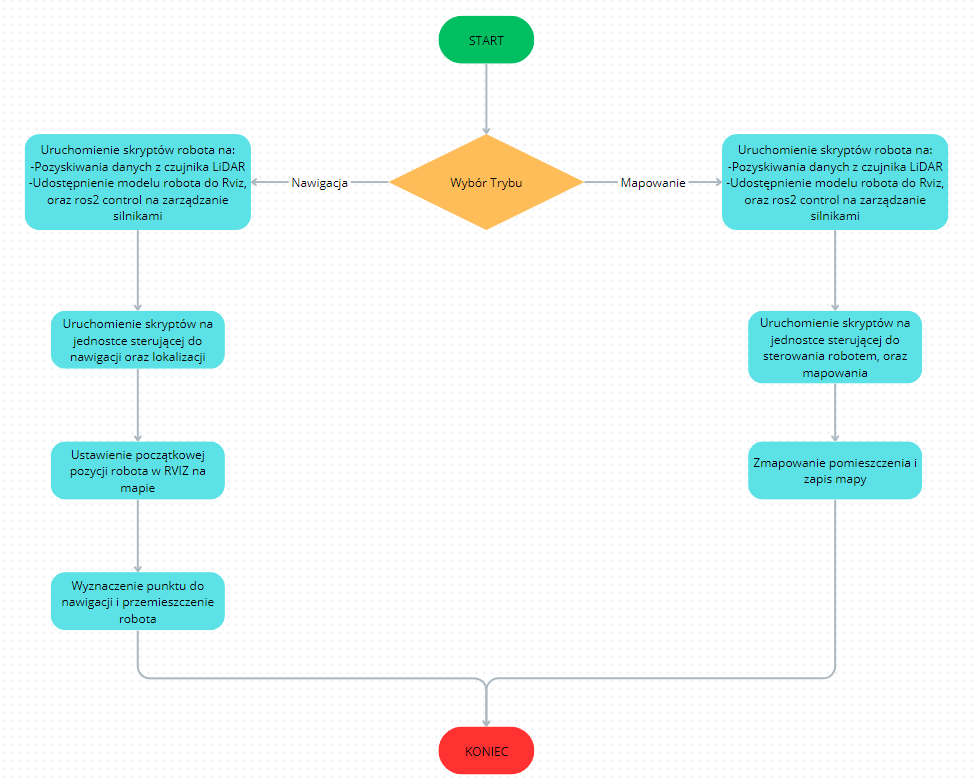
\includegraphics[width=0.8\textwidth]{images/UML.png}
\caption{Diagram przypadków użycia systemu}
\label{fig:use-case}
\end{figure}

\section{Specyfikacja komponentów}
\subsection{Jednostki sterujące}
\begin{itemize}
\item Raspberry Pi 4 - główny komputer pokładowy:
	\begin{itemize}
	\item System operacyjny Ubuntu 22.04
	\item ROS 2 Humble
	\item Komunikacja przez SSH
	\end{itemize}
\item Arduino Nano - sterownik silników:
	\begin{itemize}
	\item Obsługa enkoderów
	\item Komunikacja szeregowa z Raspberry Pi
	\end{itemize}
\end{itemize}

\subsection{Napęd}
\begin{itemize}
\item 2x silnik DC 12V 240RPM z metalową przekładnią
\item Wbudowane enkodery magnetyczne Halla
\item Sterownik L298N - dwukanałowy mostek H
\end{itemize}

\subsection{Zasilanie}
\begin{itemize}
\item 6x akumulatory Li-ion 18650:
	\begin{itemize}
	\item 4 ogniwa (2S2P) dla silników
	\item 2 ogniwa (2S) dla elektroniki
	\end{itemize}
\item 2x przetwornica step-down:
	\begin{itemize}
	\item 12V dla silników
	\item 5V dla Raspberry Pi
	\end{itemize}
\end{itemize}

\section{Metodyka i etapy realizacji}
\subsection{Etap 1: Przygotowanie platformy sprzętowej}
\begin{itemize}
\item Instalacja systemu Ubuntu 22.04 na Raspberry Pi
\item Konfiguracja połączenia SSH
\item Instalacja ROS 2 Humble
\end{itemize}

\subsection{Etap 2: Implementacja sterowania napędem}
\begin{itemize}
\item Podłączenie silników do sterownika L298N
\item Programowanie Arduino - obsługa silników i enkoderów
\item Implementacja komunikacji szeregowej z Raspberry Pi
\end{itemize}

\subsection{Etap 3: Integracja sensorów}
\begin{itemize}
\item Montaż i konfiguracja LiDAR-a
\item Kalibracja czujników
\item Opracowanie układu mechanicznego i obudowy
\end{itemize}

\subsection{Etap 4: Implementacja oprogramowania}
\begin{itemize}
\item Konfiguracja pakietów ROS 2:
	\begin{itemize}
	\item SLAM Toolbox do mapowania
	\item Nav2 do nawigacji
	\item AMCL do lokalizacji
	\end{itemize}
\item Implementacja sterowników urządzeń
\item Integracja i testy systemu
\end{itemize}



% TODO
\chapter{[Właściwy dla kierunku -- np. Specyfikacja zewnętrzna]}
\label{ch:04}

Jeśli „Specyfikacja zewnętrzna”:
\begin{itemize}
\item  wymagania sprzętowe i programowe
\item  sposób instalacji
\item  sposób aktywacji
\item  kategorie użytkowników
\item  sposób obsługi
\item  administracja systemem
\item  kwestie bezpieczeństwa
\item  przykład działania
\item  scenariusze korzystania z systemu (ilustrowane zrzutami z ekranu lub generowanymi dokumentami)
\end{itemize}

%%%%%%%%%%%%%%%%%%%%%
%% RYSUNEK Z PLIKU
%
%\begin{figure}
%\centering
%
\includegraphics[width=0.5\textwidth]{./politechnika_sl_logo_bw_pion_pl.pdf}
%\caption{Podpis rysunku zawsze pod rysunkiem.}
%\label{fig:etykieta-rysunku}
%\end{figure}
%Rys. \ref{fig:etykieta-rysunku} przestawia …
%%%%%%%%%%%%%%%%%%%%%
%
%%%%%%%%%%%%%%%%%%%%%
%% WIELE RYSUNKÓW 
%
%\begin{figure}
%\centering
%\begin{subfigure}{0.4\textwidth}
%    
\includegraphics[width=\textwidth]{./politechnika_sl_logo_bw_pion_pl.pdf}
%    \caption{Lewy górny rysunek.}
%    \label{fig:lewy-gorny}
%\end{subfigure}
%\hfill
%\begin{subfigure}{0.4\textwidth}
%    
\includegraphics[width=\textwidth]{./politechnika_sl_logo_bw_pion_pl.pdf}
%    \caption{Prawy górny rysunek.}
%    \label{fig:prawy-gorny}
%\end{subfigure}
%
%\begin{subfigure}{0.4\textwidth}
%    
\includegraphics[width=\textwidth]{./politechnika_sl_logo_bw_pion_pl.pdf}
%    \caption{Lewy dolny rysunek.}
%    \label{fig:lewy-dolny}
%\end{subfigure}
%\hfill
%\begin{subfigure}{0.4\textwidth}
%    
\includegraphics[width=\textwidth]{./politechnika_sl_logo_bw_pion_pl.pdf}
%    \caption{Prawy dolny rysunek.}
%    \label{fig:prawy-dolny}
%\end{subfigure}
%        
%\caption{Wspólny podpis kilku rysunków.}
%\label{fig:wiele-rysunkow}
%\end{figure}
%Rys. \ref{fig:wiele-rysunkow} przestawia wiele ważnych informacji, np. rys. \ref{fig:prawy-gorny} jest na prawo u góry.
%%%%%%%%%%%%%%%%%%%%%


 
\begin{figure}
\centering
\begin{tikzpicture}
\begin{axis}[
    y tick label style={
        /pgf/number format/.cd,
            fixed,   % po zakomentowaniu os rzednych jest indeksowana wykladniczo
            fixed zerofill, % 1.0 zamiast 1
            precision=1,
        /tikz/.cd
    },
    x tick label style={
        /pgf/number format/.cd,
            fixed,
            fixed zerofill,
            precision=2,
        /tikz/.cd
    }
]
\addplot [domain=0.0:0.1] {rnd};
\end{axis} 
\end{tikzpicture}
\caption{Podpis rysunku po rysunkiem.}
\label{fig:2}
\end{figure}



% TODO
\chapter{[Właściwy dla kierunku -- np. Specyfikacja wewnętrzna]}
\label{ch:05}


Jeśli „Specyfikacja wewnętrzna”:
\begin{itemize}
\item przedstawienie idei
\item architektura systemu
\item opis struktur danych (i organizacji baz danych)
\item komponenty, moduły, biblioteki, przegląd ważniejszych klas (jeśli występują)
\item przegląd ważniejszych algorytmów (jeśli występują)
\item szczegóły implementacji wybranych fragmentów, zastosowane wzorce projektowe
\item diagramy UML
\end{itemize}

% % % % % % % % % % % % % % % % % % % % % % % % % % % % % % % % % % % 
% Pakiet minted wymaga importu: \usepackage{minted}                 %
% i specjalnego kompilowania:                                       %
% pdflatex -shell-escape main                                       %
% % % % % % % % % % % % % % % % % % % % % % % % % % % % % % % % % % % 


Krótka wstawka kodu w linii tekstu jest możliwa, np.  \lstinline|int a;| (biblioteka \texttt{listings})% lub  \mintinline{C++}|int a;| (biblioteka \texttt{minted})
. 
Dłuższe fragmenty lepiej jest umieszczać jako rysunek, np. kod na rys \ref{fig:pseudokod:listings}% i rys. \ref{fig:pseudokod:minted}
, a naprawdę długie fragmenty – w załączniku.


\begin{figure}
\centering
\begin{lstlisting}
class test : public basic
{
    public:
      test (int a);
      friend std::ostream operator<<(std::ostream & s, 
                                     const test & t);
    protected:
      int _a;  
      
};
\end{lstlisting}
\caption{Pseudokod w \texttt{listings}.}
\label{fig:pseudokod:listings}
\end{figure}

%\begin{figure}
%\centering
%\begin{minted}[linenos,frame=lines]{c++}
%class test : public basic
%{
%    public:
%      test (int a);
%      friend std::ostream operator<<(std::ostream & s, 
%                                     const test & t);
%    protected:
%      int _a;  
%      
%};
%\end{minted}
%\caption{Pseudokod w \texttt{minted}.}
%\label{fig:pseudokod:minted}
%\end{figure}




% TODO
\chapter{Weryfikacja i walidacja}
\label{ch:06}
\begin{itemize}
\item sposób testowania w ramach pracy (np. odniesienie do modelu V)
\item organizacja eksperymentów
\item przypadki testowe zakres testowania (pełny/niepełny)
\item wykryte i usunięte błędy
\item opcjonalnie wyniki badań eksperymentalnych
\end{itemize}

\begin{table}
\centering
\caption{Nagłówek tabeli jest nad tabelą.}
\label{id:tab:wyniki}
\begin{tabular}{rrrrrrrr}
\toprule
	         &                                     \multicolumn{7}{c}{metoda}                                      \\
	         \cmidrule{2-8}
	         &         &         &        \multicolumn{3}{c}{alg. 3}        & \multicolumn{2}{c}{alg. 4, $\gamma = 2$} \\
	         \cmidrule(r){4-6}\cmidrule(r){7-8}
	$\zeta$ &     alg. 1 &   alg. 2 & $\alpha= 1.5$ & $\alpha= 2$ & $\alpha= 3$ &   $\beta = 0.1$  &   $\beta = -0.1$ \\
\midrule
	       0 &  8.3250 & 1.45305 &       7.5791 &    14.8517 &    20.0028 & 1.16396 &                       1.1365 \\
	       5 &  0.6111 & 2.27126 &       6.9952 &    13.8560 &    18.6064 & 1.18659 &                       1.1630 \\
	      10 & 11.6126 & 2.69218 &       6.2520 &    12.5202 &    16.8278 & 1.23180 &                       1.2045 \\
	      15 &  0.5665 & 2.95046 &       5.7753 &    11.4588 &    15.4837 & 1.25131 &                       1.2614 \\
	      20 & 15.8728 & 3.07225 &       5.3071 &    10.3935 &    13.8738 & 1.25307 &                       1.2217 \\
	      25 &  0.9791 & 3.19034 &       5.4575 &     9.9533 &    13.0721 & 1.27104 &                       1.2640 \\
	      30 &  2.0228 & 3.27474 &       5.7461 &     9.7164 &    12.2637 & 1.33404 &                       1.3209 \\
	      35 & 13.4210 & 3.36086 &       6.6735 &    10.0442 &    12.0270 & 1.35385 &                       1.3059 \\
	      40 & 13.2226 & 3.36420 &       7.7248 &    10.4495 &    12.0379 & 1.34919 &                       1.2768 \\
	      45 & 12.8445 & 3.47436 &       8.5539 &    10.8552 &    12.2773 & 1.42303 &                       1.4362 \\
	      50 & 12.9245 & 3.58228 &       9.2702 &    11.2183 &    12.3990 & 1.40922 &                       1.3724 \\
\bottomrule
\end{tabular}
\end{table}  



% TODO
\chapter{Podsumowanie i wnioski}
\begin{itemize}
\item uzyskane wyniki w świetle postawionych celów i zdefiniowanych wyżej wymagań
\item kierunki ewentualnych danych prac (rozbudowa funkcjonalna …)
\item problemy napotkane w trakcie pracy
\end{itemize}



\backmatter

%\bibliographystyle{plplain}  % bibtex
%\bibliography{biblio} % bibtex
\addcontentsline{toc}{chapter}{Bibliografia}
\printbibliography
\begin{appendices}

% TODO
\chapter{Spis skrótów i symboli}

\begin{itemize}
\item[SLAM] jednoczesna lokalizacja i mapowanie (ang. \english{Simultaneous Localization and Mapping})
\item[LiDAR] urządzenie wykonujące wykrywanie światła i określanie odległości (ang. \english{Light Detection and Ranging})
\item[IMU] inercyjna jednostka pomiarowa (ang. \english{Inertial Measurement Unit})
\item[RGB-D] kamera rejestrująca obraz RGB oraz informację o głębi (ang. \english{RGB-Depth})
\item[Nav2] system nawigacji dla ROS 2 (ang. \english{Navigation 2})
\item[ROS] system operacyjny dla robotów (ang. \english{Robot Operating System})
\item[ROS2 Control] system kontroli robotów dla ROS 2 (ang. \english{Robot Operating System 2 Control})
\item[SLAM Toolbox] zestaw narzędzi do jednoczesnej lokalizacji i mapowania (ang. \english{Simultaneous Localization and Mapping Toolbox})
\end{itemize}


% TODO
\chapter{Źródła}

Jeżeli w pracy konieczne jest umieszczenie długich fragmentów kodu źródłowego, należy je przenieść w to miejsce.

\begin{lstlisting}
if (_nClusters < 1)
	throw std::string ("unknown number of clusters");
if (_nIterations < 1 and _epsilon < 0)
	throw std::string ("You should set a maximal number of iteration or minimal difference -- epsilon.");
if (_nIterations > 0 and _epsilon > 0)
	throw std::string ("Both number of iterations and minimal epsilon set -- you should set either number of iterations or minimal epsilon.");
\end{lstlisting}


% % % % % % % % % % % % % % % % % % % % % % % % % % % % % % % % % % % 
% Pakiet minted wymaga odkomentowania w pliku config/settings.tex   %
% importu pakietu minted: \usepackage{minted}                       %
% i specjalnego kompilowania:                                       %
% pdflatex -shell-escape praca                                      %
% % % % % % % % % % % % % % % % % % % % % % % % % % % % % % % % % % % 

%\begin{minted}[linenos,breaklines,frame=lines]{c++}
%if (_nClusters < 1)
%   throw std::string ("unknown number of clusters");
%if (_nIterations < 1 and _epsilon < 0)
%   throw std::string ("You should set a maximal number of iteration or minimal difference -- epsilon.");
%if (_nIterations > 0 and _epsilon > 0)
%   throw std::string ("Both number of iterations and minimal epsilon set -- you should set either number of iterations or minimal epsilon.");
%\end{minted}


% TODO
\chapter{Lista dodatkowych plików, uzupełniających tekst pracy} 


W systemie do pracy dołączono dodatkowe pliki zawierające:
\begin{itemize}
\item źródła programu,
\item dane testowe,
\item film pokazujący działanie opracowanego oprogramowania lub zaprojektowanego i~wykonanego urządzenia,
\item itp.
\end{itemize}


\listoffigures
\addcontentsline{toc}{chapter}{Spis rysunków}
\listoftables
\addcontentsline{toc}{chapter}{Spis tabel}

\end{appendices}

\end{document}


%% Finis coronat opus.

